\documentclass[a4paper]{ctexart}
\usepackage[top=2.3cm,bottom=2cm,left=1.7cm,right=1.7cm]{geometry} 
\usepackage{amsmath} 
\usepackage{booktabs}
\usepackage{amsthm}
\usepackage{longtable} 
\usepackage{graphicx}
\usepackage{subfigure}
\usepackage{caption}
\usepackage{fontspec}
\usepackage{titlesec}
\usepackage{fancyhdr}
\usepackage{subfig}
\def\degree{$^{\circ}$}
\def\mm{\mathrm{mm}}
\def\cm{\mathrm{cm}}
\def\nm{\mathrm{nm}}
\def\V{\mathrm{V}}
\def\m{\mathrm{m}}
\def\g{\mathrm{g}}
\def\s{\mathrm{s}}
\def\i{\mathrm{i}}
\title{\textbf{复摆实验}}
\author{王崇斌 1800011716}
\date{}
\makeatletter %使\section中的内容左对齐
\renewcommand{\section}{\@startsection{section}{1}{0mm}
	{-\baselineskip}{0.5\baselineskip}{\bf\leftline}}
\makeatother
\begin{document}
	\pagestyle{fancy}
	\lhead{普通物理实验报告} 
	\chead{}
	\rhead{}
	\maketitle
    \thispagestyle{fancy}
    \section{\large{实验数据与处理}}
    \paragraph{复摆质心位置的测量结果}
    质心位置为0.00cm
    \paragraph{复摆质量的测量结果}
    复摆的质量为412.80g
    \begin{table}[htbp]
        \centering
        \caption{复摆振动周期与悬点位置关系数据表}
        \begin{tabular}{cccccc}
            \toprule[1.5pt]
            位置$x$(cm) & 20个周期总用时$t$(s) & 周期$T$(s) & 位置$x$(cm) & 20个周期总用时$t$(s) & 周期$T$(s) \\
            \midrule    
            28.20 & 25.0745 & 1.2537 & -1.20 & 60.9922 & 3.0496 \\
            27.20 & 24.9009 & 1.2450 & -2.20 & 46.9650 & 2.3483 \\
            26.20 & 24.6936 & 1.2347 & -3.20 & 39.3221 & 1.9661 \\
            25.20 & 24.5148 & 1.2257 & -4.20 & 35.0812 & 1.7541 \\
            24.20 & 24.3607 & 1.2180 & -5.20 & 31.8265 & 1.5913 \\
            23.20 & 24.2084 & 1.2104 & -6.20 & 29.7533 & 1.4877 \\
            22.20 & 24.0574 & 1.2029 & -7.20 & 28.1673 & 1.4084 \\
            21.20 & 23.9346 & 1.1967 & -8.20 & 26.9730 & 1.3486 \\
            20.20 & 23.8550 & 1.1927 & -9.20 & 26.0284 & 1.3014 \\
            19.20 & 23.7663 & 1.1883 & -10.20 & 25.3661 & 1.2683 \\
            18.20 & 23.7273 & 1.1864 & -11.20 & 24.8148 & 1.2407 \\
            17.20 & 23.7307 & 1.1865 & -12.20 & 24.4363 & 1.2218 \\
            16.20 & 23.7336 & 1.1867 & -13.20 & 24.1246 & 1.2062 \\
            15.20 & 23.8246 & 1.1912 & -14.20 & 23.9461 & 1.1973 \\
            14.20 & 23.9593 & 1.1980 & -15.20 & 23.8233 & 1.1912 \\
            13.20 & 24.1562 & 1.2078 & -16.20 & 23.7235 & 1.1862 \\
            12.20 & 24.4730 & 1.2236 & -17.20 & 23.7132 & 1.1857 \\
            11.20 & 24.8402 & 1.2420 & -18.20 & 23.7176 & 1.1859 \\
            10.20 & 25.4123 & 1.2706 & -19.20 & 23.7761 & 1.1888 \\
            9.20 & 26.0860 & 1.3043 & -20.20 & 23.8608 & 1.1930 \\
            8.20 & 27.0006 & 1.3500 & -21.20 & 23.9685 & 1.1984 \\
            7.20 & 28.1840 & 1.4092 & -22.20 & 24.0670 & 1.2033 \\
            6.20 & 29.8509 & 1.4925 & -23.20 & 24.2070 & 1.2104 \\
            5.20 & 31.9000 & 1.5950 & -24.20 & 24.3661 & 1.2183 \\
            4.20 & 35.2348 & 1.7617 & -25.20 & 24.5277 & 1.2264 \\
            3.20 & 39.3678 & 1.9684 & -26.20 & 24.7082 & 1.2354 \\
            2.20 & 47.0598 & 2.3530 & -27.20 & 24.8969 & 1.2448 \\
            1.20 & 61.0346 & 3.0517 & -28.20 & 25.1084 & 1.2554 \\
            \bottomrule[1.5pt]
        \end{tabular}
    \end{table}
    \par 
    \begin{figure}[htbp]
        \centering
        \includegraphics[scale=0.65]{data_original.eps}
        \caption{振动周期与悬点位置关系图}
    \end{figure}
    \par 
    上面给出了实验中测量的原始数据与图像,可以看出图像基本上是一个关于质心位置对称的
    曲线。
    \par 
    由复摆周期的计算公式:
    $$
    T = 2 \pi \sqrt{\frac{I_{c} + mh^{2}}{mgh}}
    $$
    其中$h$为悬点到重心之间的距离,在本实验中由于重心位置为坐标轴原点,那么$h$与前面表格中的
    位置是相同的。进一步可以得到:
    $$
    4\pi^{2}mh^{2} = g\cdot mT^{2}h - 4\pi^{2}I_{c}
    $$
    可以看出$h^{2}$与$T^{2}h$呈线性关系,由斜率即可求出$g$,由截距可以求出$I_{c}$
    \par 
    首先给出用$h>0$的数据拟合出的直线与相关参数,$r = 0.9998,\;\;g_{1} = k = 9.706\;\mathrm{m/s^{2},\;\; b = -0.4847\;\mathrm{kg\;m^{2}}}$
    \begin{figure}[htbp]
        \centering
        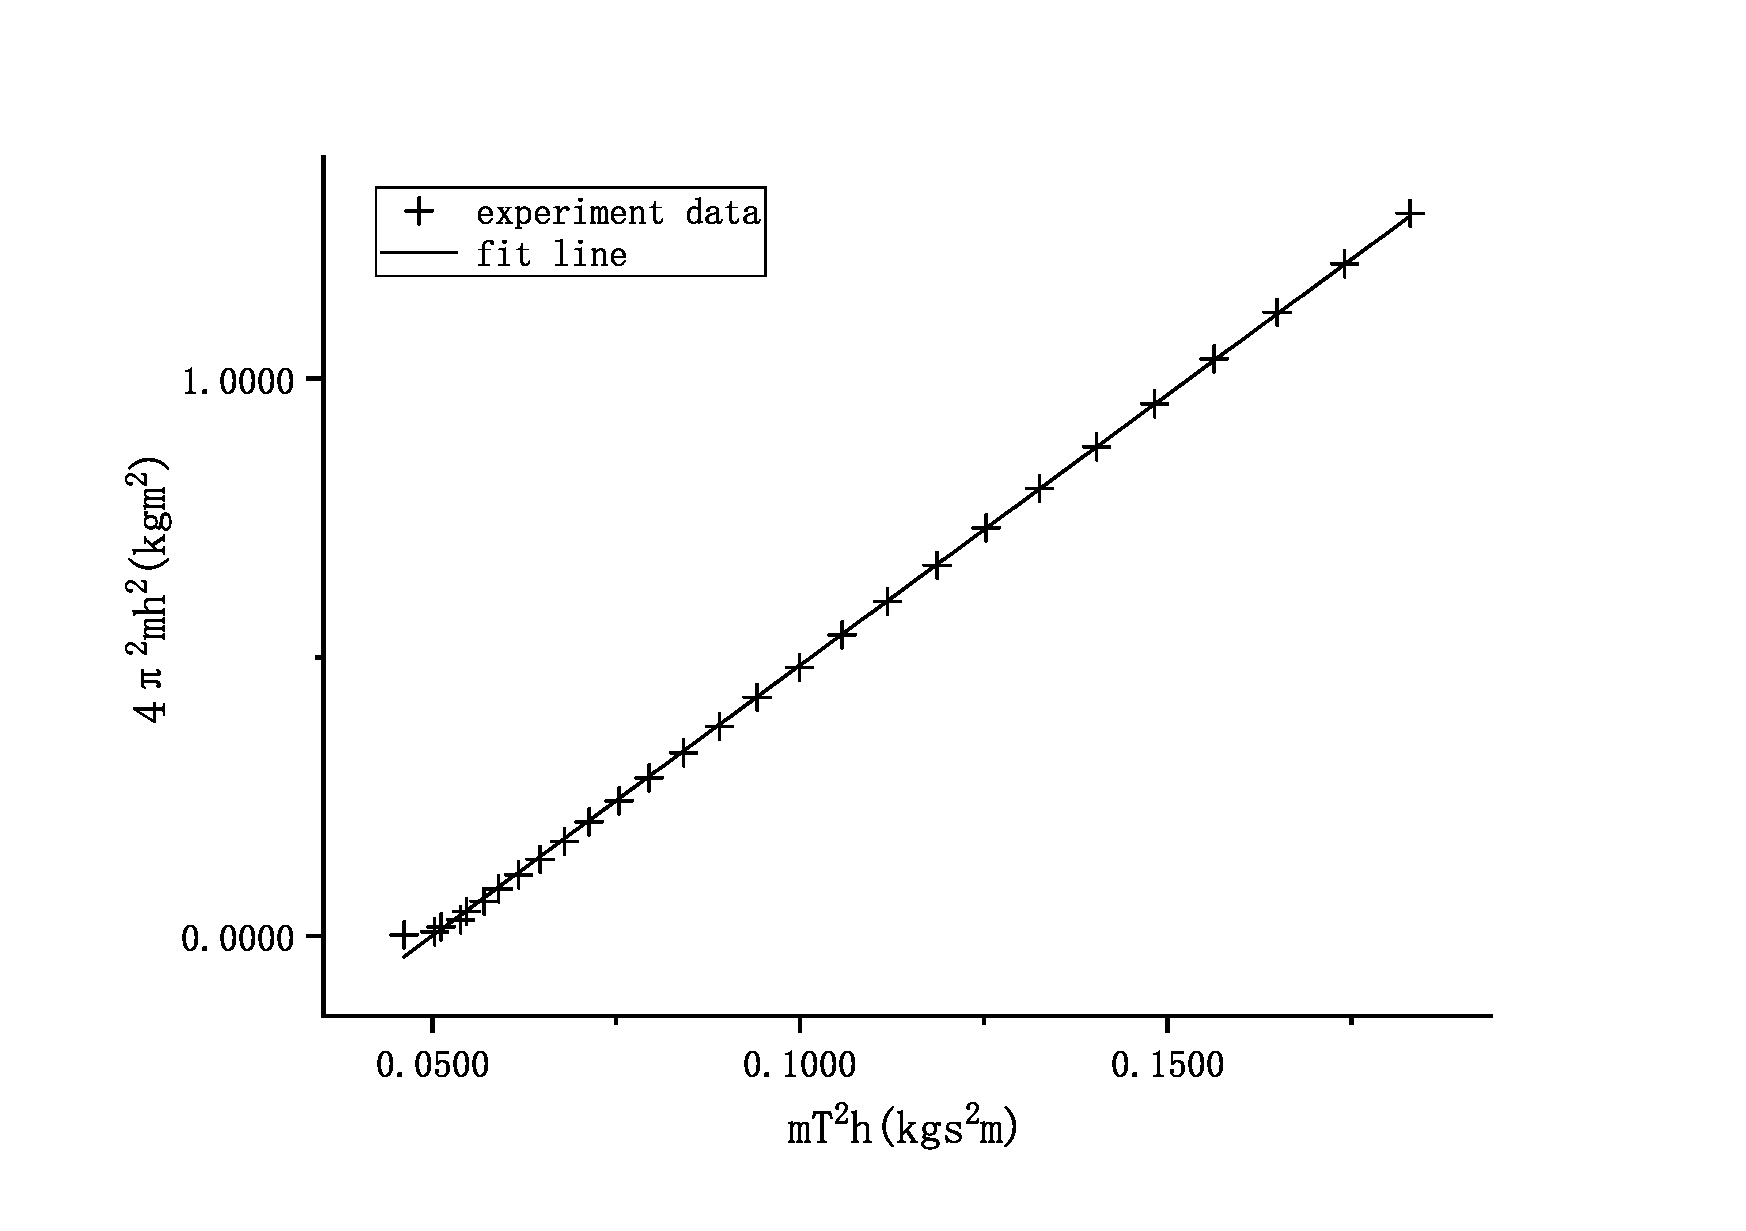
\includegraphics[scale=0.43]{h+line.eps}
        \caption{$h>0$的数据拟合直线图}
    \end{figure}
    \par 
    从图像可以看出,$h^{2}$与$T^{2}h$呈现出明显的线性关系,同时也可以看出在$h$较小
    时,数据与直线有着较为明显的偏离,这可能与$h$较小时重力提供力矩很小,摩擦力矩的
    贡献变得明显,因此出现与理论的偏离。从上面数据可以计算得到:
    $$
    I_{C1} = -\frac{b}{4\pi^{2}} = \frac{0.4847}{4\times 3.1416^{2}} = 0.01228(\mathrm{kg\;m^{2}})
    $$
    $$
    R_{C1} = \sqrt{\frac{I_{c}}{m}} = \sqrt{\frac{0.01228}{0.4128}} = 0.1725(\mathrm{m})
    $$
    \par 
    下面给出用$h<0$数据拟合出的直线与相关参数,$r = -0.9998,\;\;g_{2} = k = 9.669\;\mathrm{m/s^{2},\;\; b = 0.4805 \;\mathrm{kg\;m^{2}}}$
    \begin{figure}[htbp]
        \centering
        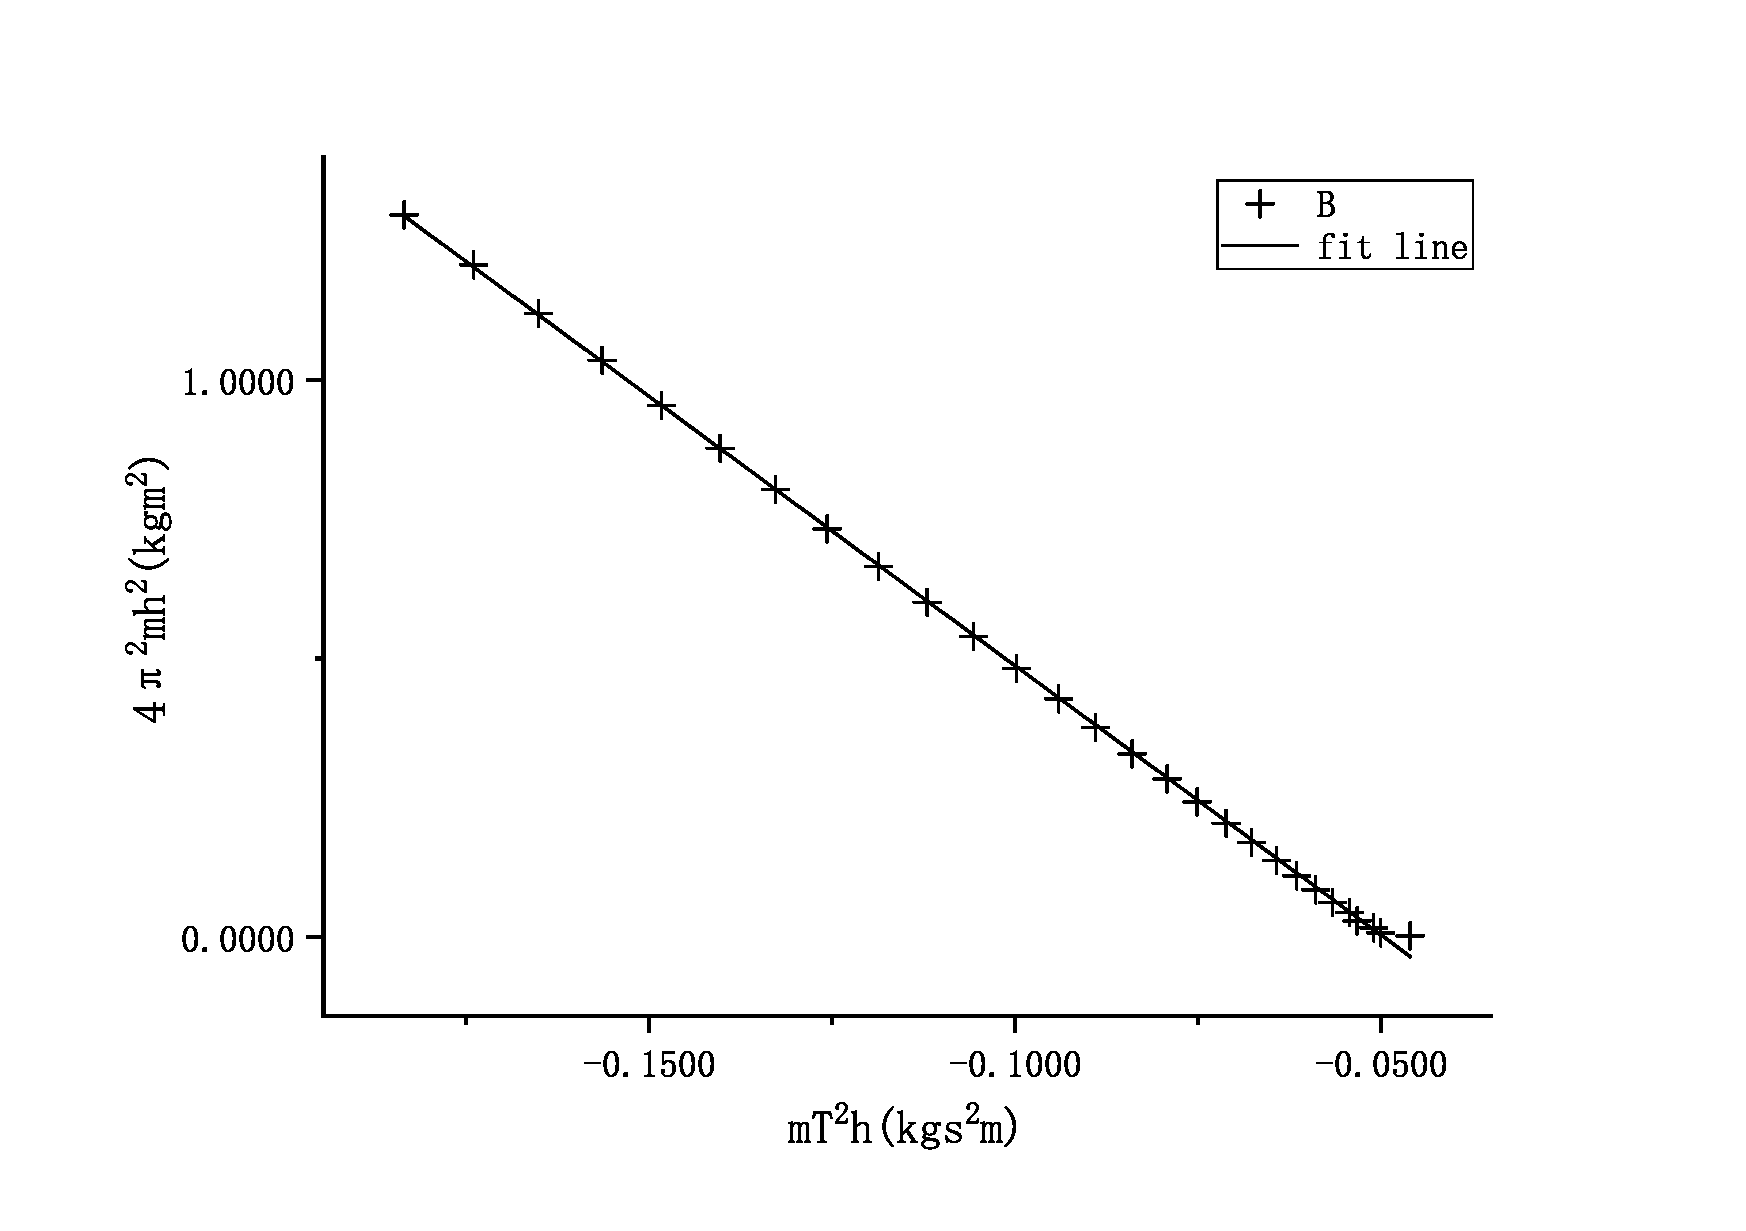
\includegraphics[scale=0.43]{h-line.eps}
        \caption{$h<0$的数据拟合直线图}
    \end{figure}
    \par 
    可以看出实验数据与拟合直线的偏离程度符合前面所述的规律,从上面的数据可以计算得到:
    $$
    I_{C2} = -\frac{b}{4\pi^{2}} = \frac{0.4805}{4\times 3.1416^{2}} = 0.01217(\mathrm{kg\;m^{2}})
    $$
    $$
    R_{C2} = \sqrt{\frac{I_{c}}{m}} = \sqrt{\frac{0.01217}{0.4128}} = 0.1717(\mathrm{m})
    $$
    \par 
    那么可以得到实验测量的重力加速度、复摆质心轴的转动惯量与回转半径分别为:
    $$
    \bar{g} = \frac{g_{1}+g_{2}}{2} = 9.69\;\mathrm{m/s^{2}}
    $$
    $$
    \bar{I_{C}} = \frac{I_{C1} + I_{C2}}{2} = 0.01222\;\mathrm{kg\;m^{2}}
    $$
    $$
    \bar{R_{C}} = \frac{R_{C1} + R_{C2}}{2} = 0.1721\;\mathrm{m}
    $$
    \par 
    下面使用近似共轭点的方法计算重力加速度,首先在测量数据中找到三组近似的共轭点。
    分别为:
    $$x = 27.20\cm,\;T = 1.2450\s\;\;x = -11.20\cm,\; T = 1.2407\s$$
    $$x = 21.20\cm,\;T = 1.1967\s\;\;x = -14.20\cm,\; T = 1.1973\s$$
    $$x = 18.20\cm,\;T = 1.1864\s\;\;x = -16.20\cm,\; T = 1.1862\s$$
    \par 
    由复摆周期公式平方相减后可得:
    $$
    \frac{4\pi^{2}}{g} = \frac{T_{1}^{2} +T_{2}^{2}}{2(h_{1} + h_{2})} + \frac{T_{1}^{2} - T_{2}^{2}}{2(h_{1}-h_{2})}
    $$
    \par 
    其中$h$为悬点到质心得距离,始终应取得正值,当我们选取了近似共轭点时,$h_{1} \neq h_{2}$
    但是$T_{1} \approx T_{2}$因此上式第二项可以忽略,由此得到:
    $$g = \frac{8\pi^{2}(h_{1} + h_{2})}{T_{1}^{2} + T_{2}^{2}}$$
    \par 
    由选择的三个共轭点可以计算出:$g_{1} = 9.814\;\mathrm{m/s^{2}},\;\;g_{2} = 9.754\;\mathrm{m/s^{2}},\;\;g_{3} = 9.650\;\mathrm{m/s^{2}}$
    $$\bar{g} = \frac{g_{1} + g_{2} + g_{3}}{3} = 9.74\;\mathrm{m/s^{2}}$$
    \par 
    接下来我们使用共轭点法来计算重力加速度,在实验曲线上寻找严格的共轭点,首先给出实验曲线与共轭点的坐标
    \begin{figure}[htbp]
        \centering
        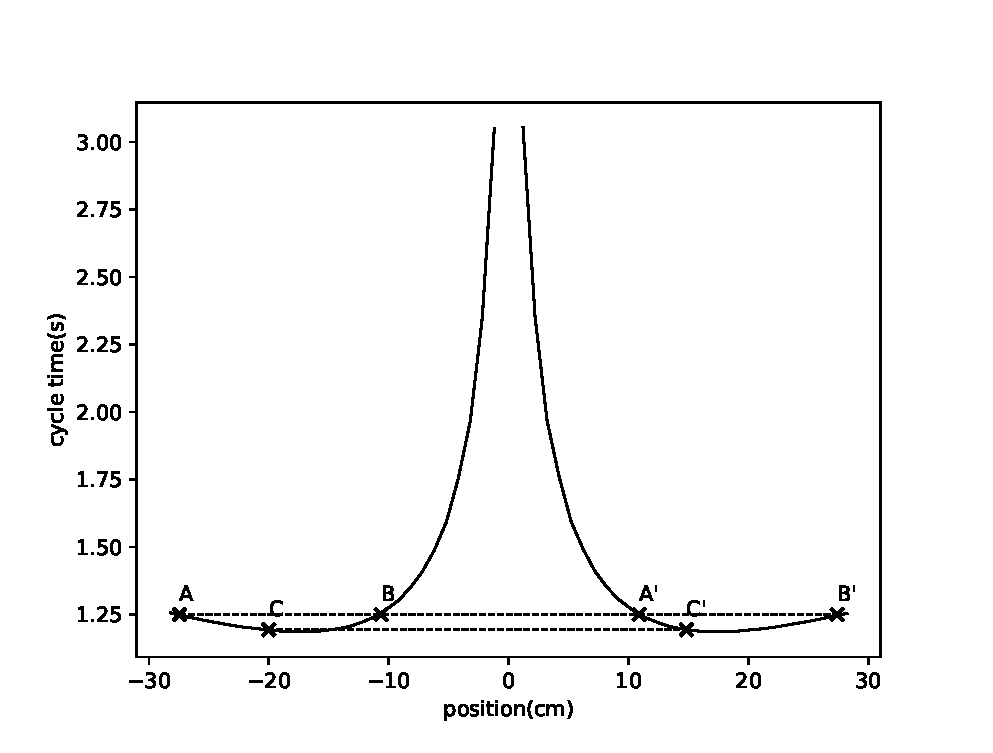
\includegraphics[scale=0.7]{conjugate_point.eps}
        \caption{实验曲线上的共轭点}
    \end{figure}
    \par 
    共轭点的坐标为:
    $$A\;(-27.46,1.2494),\;\;A^{'}\;(10.82,1.2494)$$
    $$B\;(-10.63,1.2494),\;\;B^{'}\;(27.39,1.2494)$$
    $$C\;(-20.01,1.1932),\;\;C^{'}\;(14.82,1.1932)$$
    \par 
    在这种情况下用于近似共轭点的公式严格成立,可以计算得到重力加速度:
    $g_{1}=9.681\;\mathrm{m/s^{2}},\;\;g_{2}=9.615\;\mathrm{m/s^{2}},\;\;g_{3}=9.658\;\mathrm{m/s^{2}}$
    $$
    \bar{g} \frac{g_{1} + g_{2} + g_{3}}{3} = 9.65\;\mathrm{m/s^{2}}
    $$
    \\
    \section{\large{实验收获}}
    \par 
    本次实验中由于自己的疏忽导致误以为自己的实验数据测量错误而重测了很多组数据,这也直接导致了实验
    超出了预期的时间,在这里给老师道歉。这就提醒我实验时一定要想清楚自己自己在干什么,不能机械地做实验
    ;同时还有实验数据记录的问题,不要把自己认为错误的实验数据全部涂掉,有可能这些数据还有用处。
\end{document}
